
\title{Recap Computer Architectures (02LSEOV)}
\author{Jacopo Nasi\\
        Computer Engineer\\
        Politecnico di Torino}
\date{I Period - 2017/2018\\\bigskip\bigskip\today}

\documentclass[12pt]{article}
\usepackage[utf8]{inputenc}
\usepackage[italian]{babel}
\usepackage{geometry}
\usepackage{indentfirst} % First line indent
\usepackage{mathtools}
\usepackage{wrapfig}
\usepackage[usenames, dvipsnames]{color}
\usepackage{float}
\usepackage{amssymb}
\usepackage{ifsym}
% Misure Documento
\geometry{ a4paper, total={170mm,257mm},left=35mm, right=35mm, top=35mm, bottom=35mm }

\begin{document}

\begin{figure}
  \centering
  
\includegraphics[width=10cm]{images/polito.pdf}
\end{figure}

\maketitle

\newpage
\tableofcontents

\newpage
{\noindent \Large \textbf{License}\bigskip}

This work is licensed under a Creative Commons Attribution-NonCommercial-ShareAlike 3.0 Unported License.\\
You are free:
\begin{itemize}
  \item \textbf{to Share}: to copy, distribute and transmit the work
  \item \textbf{to Remix}: to adapt the work
\end{itemize}
Under the following conditions:
\begin{itemize}
  \item \textbf{Attribution}: you must attribute the work in the manner specified by the author or licensor (but not in any way that suggests that they endorse you or your use of the work)
  \item \textbf{Noncommercial}: you may not use this work for commercial purposes.
  \item \textbf{Share Alike}: if you alter, transform, or build upon this work, you may distribute the resulting work only under the same or similar license to this one.
\end{itemize}

\noindent More information on the Creative Commons website (http://creativecommons.org).

\begin{figure}[h!]
  \centering
  
\includegraphics[width=3cm]{images/license.png}
\end{figure}

{\noindent \Large \textbf{Acknowledgments}\bigskip}

Questo breve riepilogo non ha alcuno scopo se non quello di agevolare lo studio di me stesso, se vi fosse di aiuto siete liberi di usarlo.\\
Le fonti su cui mi sono basato sono quelle relative al corso offerto (\textbf{Computer Architectures (02LSEOV)}) dal Politecnico di Torino durante l'anno accademico 2017/2018.\\
Non mi assumo nessuna responsabilità in merito ad errori o qualsiasi altra cosa. Fatene buon uso!
\newpage

\section{Introduction Computer Design}
\subsection{Computer Evolution}
The first general-purpose computer was created in the late 40s. What now we can buy for 500\$ is equivalent (performance) to what could be bought for about \$1M in 85'.\\
During the years the performance growth was not linear, as you can see in figure , during the first 10 years the annual increase was around 25-30\%/year, from the late 80s to the 2000 the growth is increased around 50\%/year and, in the last few years it decrease to the 22\%. Why this change during the increase?\\
\begin{figure}[h!]
  \centering
  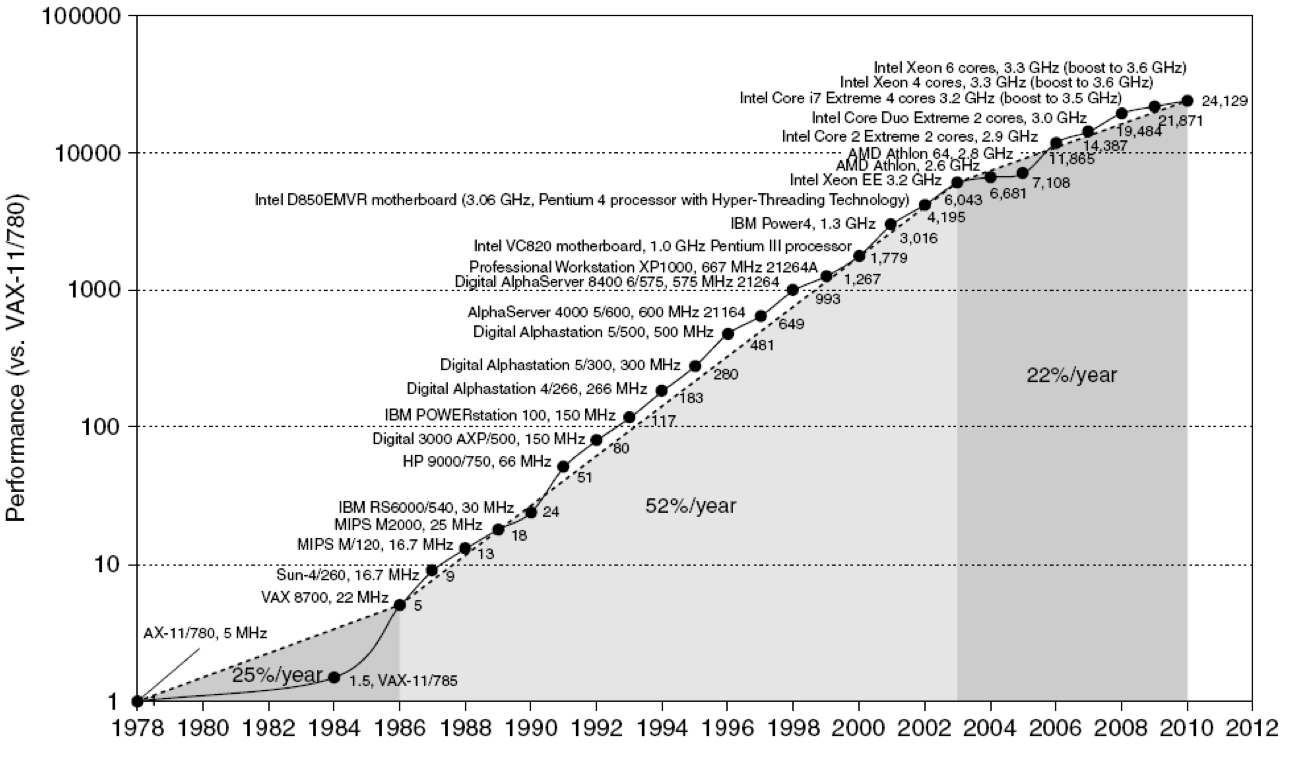
\includegraphics[width=3cm]{images/cpugrowth.png}
\end{figure}
The manufacturers have found a lot of physical problem related to the creation of new products, this problem are mainly related to:
\begin{itemize}
  \item Power-Issue.
  \item Lower instruction-level parallelism.
  \item Unchanged memory lantecy.
\end{itemize}
in fact, since 2004, the major industry have changed the conceptual ways to desing processors, switching from single to multi-core architectures. We can say that, in anytime, this growth is incredible an is due to improvements in technology, microprocessor architecture and software development. %Intro @ Pag. 10


\bibliographystyle{abbrv}
\bibliography{simple}

\end{document}
